\newcommand{\Draft}{}
\newcommand{\Slide}{}
\newcommand{\PrintLecture}{1}
\newcommand{\PrintSolution}{1}
\newcommand{\MyCourse}{データサイエンスコース}
\newcommand{\MySemester}{春}
\newcommand{\MySubject}{ビジネス アナリティクス}
\newcommand{\MyClass}{第17回ー分類}% フォルダ名自動挿入

%
% 科目共通定義
%

\newcommand{\OpenIntro}
{\MyRef{OpenIntro Statistics}{https://www.openintro.org/book/os}}

\newcommand{\R}{\textbf{R}}
\newcommand{\RStudio}{\textbf{RStudio}}
\newcommand{\Excel}{\textbf{Excel}}
\newcommand{\cs}[1]{\textcolor{blue}{\texttt{#1}}} % Console prompt >

\newcommand{\ra}{\rightarrow}
\newcommand{\Ra}{\Rightarrow}

% Expectation E[X]
\def\E#1{E\big[#1\big]}
\def\S{\sum_{i=1}^n}

\newcommand{\B}{\hat{\beta}}
\newcommand{\SUM}{\sum_{i=1}^n}  % Summention from i=1 to n
\newcommand{\NH}{$\mathit{H}_0$} % Null hypthesis
\newcommand{\AH}{$\mathit{H}_1$} % Alternative hypothesis
\newcommand{\T}{\texorpdfstring{$t$}{}}% Student's t
\newcommand{\overtext}[3][1.5]{
  \mathrel{\overset{#2}{\scalebox{#1}[1]{$#3$}}}
}
\newcommand{\iid}{\overtext[2]{iid}{\sim}}
\newcommand{\convdist}{\overtext[2]{d}{\rightarrow}}
\newcommand{\convprob}{\overtext[2]{p}{\rightarrow}}
\newcommand{\as}[2]{\quad \text{as}\quad #1 \rightarrow #2}

\input{../../tex/hss_lualatex.tex}
\input{../../tex/hss_hyperref.tex}
\input{../../tex/hss_beamer.tex}

\setbeameroption{hide notes}
%\setbeameroption{show notes}
%\setbeameroption{show only notes}
%\setbeameroption{show notes on second screen=right}

\begin{document}

\maketitle

\MyFrame{}{\tableofcontents}

\section{決定係数}

\MyFrame{}
{
  \MyFig{1.1}{coef_determination1.png}
  \MyRef{BellCurve 統計WEB}
  {https://bellcurve.jp/statistics/course/9706.html}
}

\MyFrame{}
{
  \MyFig{0.4}{coef_determination2.png}
  \MyRef{BellCurve 統計WEB}
  {https://bellcurve.jp/statistics/course/9706.html}
}

\MyFrame{}
{
  平均からの全変動は回帰変動と残差変動に分解できる。
  \[\underbrace{\sum(y_i-\bar{y})^2}_{全変動}
    =\underbrace{\sum(\hat{y}_i-\bar{y})^2}_{回帰変動}
    +\underbrace{\sum(y_i-\hat{y})^2}_{残差変動}\]
    決定係数は全変動に含まれる回帰変動の割合を示している。
    つまり,目的変数を回帰モデルでどのぐらい説明できるか
    という度合いを示しておりモデル性能を測る指標である。
    決定係数は\MyFill{\ruby{寄与率}{きよりつ}}とも呼ばれる。
  \[決定係数 R^2=\frac{回帰変動}{全変動}
    =\frac{\sum(\hat{y}_i-\bar{y})^2}{\sum(y_i-\bar{y})^2}\]
  \[R^2=\frac{回帰変動}{全変動}
    =\frac{全変動-残差変動}{全変動}=1-\frac{残差変動}{全変動}
    =1-\frac{\sum(y_i-\hat{y})^2}{\sum(y_i-\bar{y})^2}\]
}

\MyFrame{決定係数の値域}
{
  最小二乗法で得られた回帰モデルでは必ず$0\le R^2 \le 1$となる。
  最小二乗法を使わない任意の数理モデルの場合で
  $R^2=1-\frac{残差変動}{全変動}$ の式で決定係数を計算したときには
  $R^2 <0$となる場合もある。
  \MyFig{0.5}{R/negative_coef_determination.png}
}

\MyFrame{自由度調整済み決定係数$adj.R^2$}
{
  全変動,残差変動をそれぞれの自由度割った決定係数を
  \MyFill{自由度調整済み決定係数}という。$adj.R^2$や$R_f^2$と表記される。
  \[adj.R^2
    =1-\frac{残差変動/残差変動の自由度}{全変動/全変動の自由度}
    =1-\frac{\frac{\sum(y_i-\hat{y})^2}{n-p-1}}
            {\frac{\sum(y_i-\bar{y})^2}{n-1}}\]
  ここで,$n,p$はそれぞれ,標本サイズ,説明変数の数である。
  説明変数の数が異なる複数の回帰モデルを比較するときに用いる指標である。
}

\MyFrame{AIC}
{
  統計数理研究所の赤池弘次所長が考案した情報量基準
  AIC(Akaike Information Criterion)\\
  \[AIC=-2L+2p\]
  ここで,
  $L$:モデルの最大\ruby{対数尤度}{たいすうゆうど},
  $p$:モデルの説明変数の数\\
  AICは値が小さければ小さいほど良い予測モデルとなる。
  \ruby{交差検証法}{こうさけんしょうほう}で評価しているのと漸近的に等価である。
  %AIC is asymptotically equivalent to leave-1-out cross-validation (LOOCV) (Stone 1977) 
  %BIC is equivalent to leave-k-out cross-validation (LKOCV) where k=n[1−1/(log(n)−1)], with n= sample size (Shao 1997)
}

\section{\ruby{過学習}{かがくしゅう}}

\MyFrame{\insertsection}
{
  回帰分析に使用する説明変数の数$p$に比べて
  標本サイズ$n$が著しく少ない場合に,次に示す
  \MyFill{\ruby{過学習}{かがくしゅう}(\ruby{過適合}{かてきごう})}
  と呼ばれる問題が発生する。
  この問題を回避するには,回帰係数の数($p+1$)の
  \MyFill{10倍}以上の標本サイズ(学習データサイズ)
  $n\ge10(p+1)$が必要とされている(経験則)。
}

\newcounter{x}
\forloop{x}{1}{\value{x}<11}
{
  \MyFrame{\insertsection 回帰係数の数($p+1$):\arabic{x}}
  {
    \MyFig{0.75}{./R/overfitting_\arabic{x}.pdf}
  }
}

\MyFrame{\insertsection まとめ}
{
  過学習が起こると観測値に非常に近い値を出すが
  真のモデルとは程遠いモデルとなる。
  このため,予測時の\ruby{大外}{おおはず}しの原因となる。
  回帰係数の数と標本サイズが同じ($p+1=n$)になると
  観測値と適合値は完全に一致する。
  逆に,回帰係数の数が1,2のときはモデルの表現力が不足しており
  \MyFill{未学習}(underfitting)と呼ばれる。\\
  自由度調整済み決定係数やAICは標本サイズが
  本例のようにとても小さいとモデル評価に使えないことが分かる。\\
  過学習の対策としては,標本サイズを大きくすることや,
  より単純なモデルを採用することの他に,
  \MyFill{\ruby{正則化}{せいそくか}}(normalization),
  \MyFill{\ruby{交差検証法}{こうさけんしょうほう}}
  (CV; cross validation)などがある。
}

\section{\ruby{変数選択法}{へんすうせんたくほう}}

\MyFrame{\insertsection}
{
  本来不要な説明変数が多いと
  それぞれの説明変数の影響が重なり合い
  思わぬ結果がでしまうことがある。
  不要な説明変数はできるだけ除くことが望ましい。
  変数選択(特徴量選択)には次の3つの主な方法がある。
  \MyEnums
  {
    \item \ruby{変数指定法}{へんすうしていほう}・・・ドメイン知識により必要な説明変数を指定する方法(最も分かりやすい)
    \item \ruby{総当り法}{そうあたりほう}・・・全ての説明変数の組み合わせを網羅し最も良い説明変数を選択する方法。(計算コストが高い)
    \item \ruby{逐次選択法}{ちくじせんたくほう}・・・一定の規則に従って説明変数を逐次選択していく方法。(計算コストを抑えつつ自動で選択する)
  }
}

\MyFrame{逐次選択法の種類}
{
  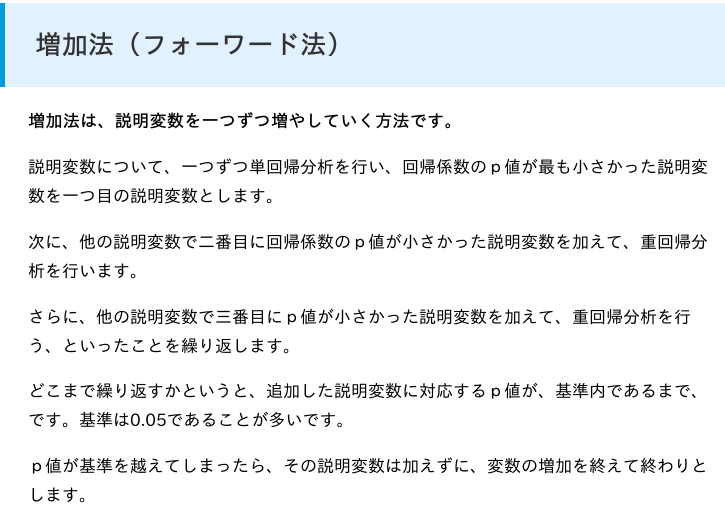
\includegraphics[width=\textwidth]{forward.png}
  \MyRef
  {統計学がわかった!}
  {https://toukeigaku-jouhou.info/2019/07/20/variable-selection-procedure}
}

\MyFrame{逐次選択法の種類}
{
  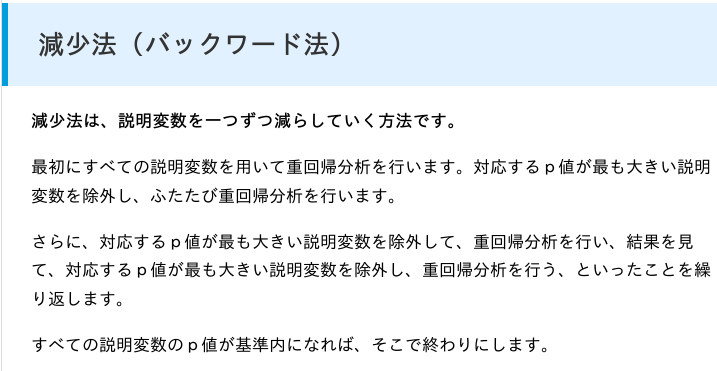
\includegraphics[width=\textwidth]{backward.png}
  \MyRef
  {統計学がわかった!}
  {https://toukeigaku-jouhou.info/2019/07/20/variable-selection-procedure}
}

\MyFrame{逐次選択法の種類}
{
  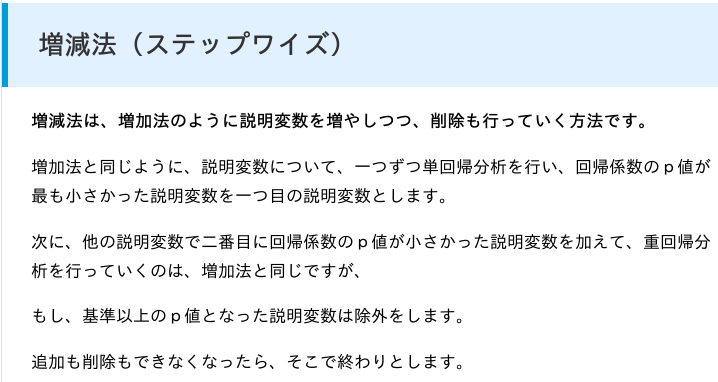
\includegraphics[width=\textwidth]{stepwise.png}
  \MyRef
  {統計学がわかった!}
  {https://toukeigaku-jouhou.info/2019/07/20/variable-selection-procedure}
}

\MyFrame{変数選択法を利用するときの注意}
{
  変数選択法は,全く本来因果関係のない変数が
  選択される場合があり合理的な解釈に苦しむことがある。
  理想的には,ドメイン知識をもとに回帰分析前に
  必要となる説明変数を決める方が良い。
  総当り法や逐次選択法では分析者が今まで気づかなかった
  有効な変数や特徴量を発見することもある。
}

\MyFrame{変数選択が不必要/必要な場合}
{
  \MyFig{1.0}{why_variable_selection.png}
  \MyRef{総務省統計局 第2講}
  {https://www.stat.go.jp/teacher/dl/pdf/c3learn/materials/third/dai2.pdf}
}

\appendix

\section{標本サイズを大きくして過学習を防止した例}

\forloop{x}{1}{\value{x}<11}
{
  \MyFrame{【付録】回帰係数の数($p+1$):\arabic{x},$n=100$}
  {
    \MyFig{0.75}{./R/overfitting_\arabic{x}n100.pdf}
  }
}

\MyFrame{【付録】まとめ}
{
  自由度調整済み決定係数やAICは,
  回帰係数の数が3のときに,
  それぞれ数字が最も大きく($adj.R^2=0.55$),小さく($AIC=-383$)なっており
  正しくモデル性能を評価できている。
}

\MyFrame{ありがちな間違い}
{
  訓練データでモデルを学習させ,
  また同じ訓練データで予測精度を評価してしまう誤り。
  \ra 訓練データとテストデータを分けることが必要。
}

\MyFrame{汎化性能}
{
  \MyDefinition{\ruby{汎化性能}{はんかせいのう}}
  {
    未知のデータに対する予測能力のことを
    \ruby{汎化性能}{はんかせいのう}という。
    過学習モデルは,この性能が低い。
    いかに訓練データに過学習することなく汎化性能を高めるかが
    良い予測モデル作成のためにとても重要である。
    データサイエンティストの腕の見せ所でもある。
  }
}

\MyFrame{スパース線形回帰による変数選択}
{
  LASSO回帰では,回帰係数の推定と変数選択を同時に行う効率的な手法。 
  予測に寄与しない説明変数の回帰係数がゼロになる(スパース性)ことで
  変数選択を自動で行う。
}

\MyFrame{ランダムフォレストによる変数選択}
{

  \MyRef{ランダムフォレストと検定を用いた特徴量選択手法 Boruta}
  {https://aotamasaki.hatenablog.com/entry/2019/01/05/195813}
}

\MyFrame{Bias Variance Trade Off}
{

}

\MyFrame{特徴量エンジニアリング}
{

}

\MyFrame{}
{

The three most common Cross-Validation Techniques are:

    Leave one out cross-validation (LOOC)
    K-fold cross-validation
    repeated k-fold cross validation.
}




\end{document}
